% =========================================================================== %
% Yes. This is a document.

\documentclass[
	english,
	aspectratio=169,
	table
]{beamer}

% =========================================================================== %
% Theme
\usepackage{scrlfile}
	\ReplacePackage{beamerthemeSHUR}{./sty/beamerthemeSHUR}
	\ReplacePackage{beamerinnerthemefancy}{./sty/beamerinnerthemefancy}
	\ReplacePackage{beamerouterthemedecolines}{./sty/beamerouterthemedecolines}
	\ReplacePackage{beamercolorthemechameleon}{./sty/beamercolorthemechameleon}

\usetheme[
	pageofpages=von,
	bullet=circle,
	titleline=true,
	alternativetitlepage=true,
	watermark="",
	watermarkheight=0px,
	watermarkheightmult=0
	]
{SHUR}

% =========================================================================== %
% the usual stuff

\usepackage[utf8]{inputenc}
\usepackage[T1]{fontenc}
\usepackage{babel}
\usepackage{lmodern}
\usepackage{microtype}
\usepackage{csquotes}

\usepackage{tabularx}
\usepackage{booktabs}
\usepackage{multirow}

\usepackage{color, colortbl}
\usepackage{xcolor}
	\definecolor{tabhighlight}{RGB}{230,240,255}
	\definecolor{tabcontrast} {RGB}{200,210,255}

\usepackage{tabto}
\usepackage{xspace}

% math
\usepackage{amsmath}
\usepackage{amssymb}
\usepackage{dsfont}
\usepackage[arrowdel]{physics}
\usepackage{mathtools}
\usepackage{siunitx}

\usepackage{minted}
	\usemintedstyle{friendly}

\usepackage{tikz}
	\usetikzlibrary{positioning}
	\usetikzlibrary{matrix}
	\usetikzlibrary{shapes.geometric}
	\usetikzlibrary{backgrounds}
	\usetikzlibrary{calc}
	\usetikzlibrary{decorations.pathreplacing}
	\usetikzlibrary{arrows}
\usepackage{adjustbox}

\usepackage[most]{tcolorbox}
	\tcbsetforeverylayer
		{colback=cyan!10!white,
		 colframe=cyan!75!black,
		 arc=0pt,
		 outer arc=0pt,
		 parbox=false
		}
	\newtcolorbox{codebox}[1][Code]
		{colback=black!5!white,
		 colframe=blue!40!black,
		 title=#1,
		 leftupper=6mm
		}
	\newtcolorbox{cmdbox}[1][Kommandozeilen-Befehl]
		{colback=black,
		 coltext=white,
		 fontupper=\ttfamily ,
		 colframe=blue!40!black,
		 title=#1,
		 outer arc=0pt
		}
	\newtcolorbox{warnbox}[1][Beachte]
		{colback=black!5!white,
		 colframe=red!40!black,
		 title=#1
		}
	\newtcolorbox{hintbox}[1][Tipp]
		{colback=black!5!white,
		 colframe=green!40!black,
		 title=#1
		}
	\newenvironment{itembox}
		{\begin{tcolorbox}\begin{itemize}}%
		{\end{itemize}\end{tcolorbox}}
	\newtcolorbox{doublebox}[1][.3]
		{righthand width=#1\linewidth,
		 sidebyside,
		 sidebyside gap=6mm,
		 sidebyside align=center,
		 lower separated=false}
	
%==============================================================================%
% GLOBAL MACROS

\newcommand*{\eg}{e.\,g. }
\newcommand*{\ie}{i.\,e. }

\newcommand{\Thus}{\ensuremath{\Rightarrow}\xspace}
\newcommand{\thus}{\ensuremath{\rightarrow}\xspace}

\newcommand*{\tabcrlf}{\\ \midrule}			% actually still allows for optional argument

\newcommand*{\inPy}[1]{\mintinline{python3}{#1}}

% =========================================================================== %

\author{Stefan Hartinger}
\title{Programming in Python}
\subtitle{Part 11: The MatPlotLib}
\institute{University Regensburg, Department of Theoretical Physics}
\date{Block Course, Summer Term 2021}

% =========================================================================== %

\begin{document}
% =========================================================================== %

\begin{frame}[t,plain]
\titlepage
\end{frame}

% =========================================================================== %

\begin{frame}{Recap}
%
\begin{columns}[T]
\column{.5\linewidth}
\begin{itemize}
\item Exceptions
\item Block structure
	\begin{itemize}
	\item \inPy{try}: Anything that might go wroing
	\item \inPy{except}: What to do if something goes wrong
	\item \inPy{else}: What to do if everything is all right
	\item \inPy{finally}: What to do in any case
	\end{itemize}
\item Error Classes
	\begin{itemize}
	\item Hierarchical Order
	\item Allows specific treatment
	\end{itemize}
\end{itemize}
%
\column{.5\linewidth}
\begin{itemize}
\item Command \inPy{raise}
	\begin{itemize}
	\item Trigger an exception yourself
	\item Argument: instance of an error class
	\item Or: Re-raise in an \inPy{except} block
	\end{itemize}
\item Own Error Classes
	\begin{itemize}
	\item Inherit from \texttt{Exception}
	\item Arbitrary Design
	\item Usually only for specific treatment of user-defined errors: \enquote{empty} classes
	\end{itemize}
\end{itemize}

\end{columns}
%
\begin{center}
	\emph{Any Questions?}
\end{center}
%
\end{frame}

% =========================================================================== %

\begin{frame}{Recap}
%
\begin{columns}[T]
\column{.5\linewidth}
\begin{itemize}
\item Manipulating the file cursor
	\begin{itemize}
	\item \texttt{handle.tell} -- get current position
	\item \texttt{handle.seek(offset, startPoint)} -- move file cursor
	\end{itemize}
\item Pickle
	\begin{itemize}
	\item Serialize objects
	\item Works with (virtually) everything in Python
	\item May contain (harmful) code
	\item \texttt{pickle.dump} and \texttt{pickle.load}
	\end{itemize}
\end{itemize}
%
\column{.5\linewidth}
\begin{itemize}
\item JSON
	\begin{itemize}
	\item Inter-Plattform serialization
	\item Only works with specific data types
	\item Human readable format
	\item \texttt{json.dump} and \texttt{json.load}
	\item Usually: \inPy{dict}s of variables
	\end{itemize}
\item CSV
	\begin{itemize}
	\item Data in columns
	\item Class \texttt{DictReader} via \texttt{csv.reader}
	\item Iterable -- can be used with \inPy{for}
	\item Rows split into columns by a separator character (\eg \texttt{','}) into \inPy{list}s
	\end{itemize}
\end{itemize}

\end{columns}
%
\begin{center}
	\emph{Any Questions?}
\end{center}
%
\end{frame}

% =========================================================================== %

\begin{frame}[fragile]
%
\begin{tcbraster}[raster columns=2,
                  raster equal height,
                  nobeforeafter,
                  raster column skip=0.5cm]
\begin{codebox}[Example: Title goes here]
\begin{minted}[fontsize=\scriptsize, linenos]{python}
foo
\end{minted}
\end{codebox}
%
\begin{codebox}[Example: Title goes here]
\begin{minted}[fontsize=\scriptsize, linenos]{python}
bar
\end{minted}
\end{codebox}
\end{tcbraster}
%
\end{frame}

% =========================================================================== %

\begin{frame}[fragile]{Chapter 10}
%
\begin{itemize}
\item Basics of the MatPlotLib
\item Manipulating Plot Details
\item Different Plot Types
\item Object Oriented Approac
\item 3D Plots
\item Saving Plots into Files
\end{itemize}
%
\end{frame}

% =========================================================================== %

\begin{frame}[fragile]{A First Example}
%
\begin{codebox}[Example: A Simple Plot, width=.53\linewidth, nobeforeafter, equal height group = grpXmpSimplePlot]
\begin{minted}[linenos, fontsize=\scriptsize]{python3}
import math
import matplotlib.pyplot as plt

N = 100
X = [(x - N/2) / 10 for x in range(N)]
Y = [math.sin(x) for x in X]

plt.plot(X, Y)
plt.show()
\end{minted}
\end{codebox}
%
\begin{tcolorbox}[title=Output: A Simple Plot, width=.45\linewidth, nobeforeafter, equal height group = grpXmpSimplePlot]
	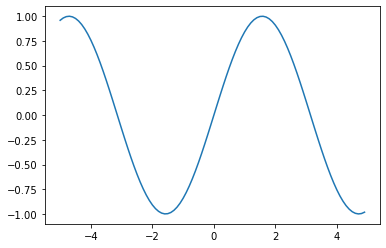
\includegraphics[width=\linewidth]{./gfx/plt-sin}
\end{tcolorbox}
%
\end{frame}

% =========================================================================== %

\begin{frame}[fragile]{Code Analysis}
%
\begin{itemize}
\item \inPy{import matplotlib.pyplot as plt}
	\begin{itemize}
	\item Module \texttt{matplotlib.pyplot} brings tons of functions
	\item Highly complex structure -- organized into sub-modules
	\item Convention: load as \texttt{plt} to spare us typing this over and over
	\end{itemize}
\item Objects \texttt{X, Y}
	\begin{itemize}
	\item Data to plot
	\item Simple lists of numbers
	\item Same length
	\item Coordinates
	\end{itemize}
\item \inPy{plt.plot(X, Y)}
	\begin{itemize}
	\item Prepare the plot in memory
	\item Allows for alterations to the default settings
	\end{itemize}
\item \inPy{plt.show()}
	\begin{itemize}
	\item \enquote{Go live}
	\item Show the plot on screen
	\item Wait with execution until plot window is closed
	\end{itemize}
\end{itemize}
%
\end{frame}

% =========================================================================== %

\begin{frame}[fragile]{Adding Some Details}
%
\begin{codebox}[Example: Plot with Grid and Legend, width=.49\linewidth, nobeforeafter, equal height group = grpXmpGrid]
\begin{minted}[linenos, fontsize=\scriptsize]{python3}
import math
import matplotlib.pyplot as plt

N  = 100
X  = [(x - N/2) / 10 for x in range(N)]
Y1 = [math.sin(x) for x in X]
Y2 = [math.cos(x) for x in X]

plt.plot(X, Y1, label="Sinus")
plt.plot(X, Y2, label="Cosinus")

plt.legend()
plt.grid()

plt.show()
\end{minted}
\end{codebox}
%
\begin{tcolorbox}[title=Output: Plot with Grid and Legend, width=.49\linewidth, nobeforeafter, equal height group = grpXmpGrid]
	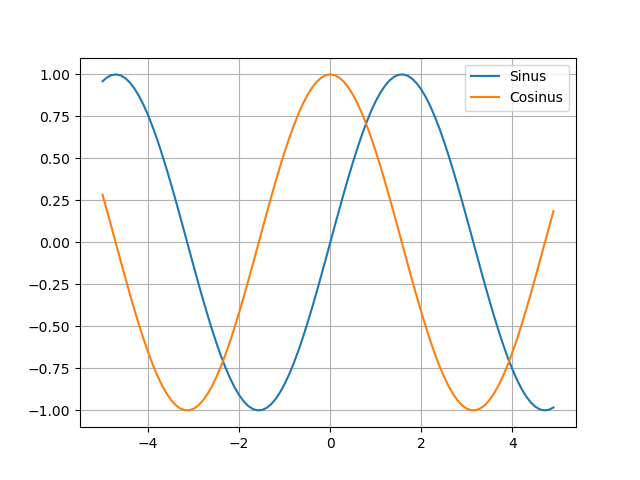
\includegraphics[width=\linewidth]{./gfx/plt-grid}
\end{tcolorbox}
%
\end{frame}

% =========================================================================== %

\begin{frame}[fragile]{Code Analysis}
%
\begin{itemize}
\item Multiple \texttt{plt.plot} lines
	\begin{itemize}
	\item Simply adds multiple lines
	\item Automatically picks new color for each new line
	\end{itemize}
\item Optional argument \texttt{label}
	\begin{itemize}
	\item Text to put in the legend
	\item By default: empty string
	\item Not automatically displayed!
	\end{itemize}
\item \inPy{plt.leged()}
	\begin{itemize}
	\item Show a box with line colour and labels
	\end{itemize}
\item \inPy{plt.grid()}
	\begin{itemize}
	\item Show a grid
	\end{itemize}
\end{itemize}
%
\end{frame}

% =========================================================================== %

\begin{frame}[fragile]
%
\begin{codebox}[Example: Headline and Axis Labels]
\begin{minted}[linenos, fontsize=\scriptsize]{python3}
import math
import matplotlib.pyplot as plt

h  = 6.62607015e-34     # Planck constant
T  = 300                # temperature in Kelvin
c  = 299792458          # speed of light
kB = 1.380649e-23       # Boltzmann constant

spectralDensity = lambda nu : ((2 * h * nu**3) / (c**2))  / \
                              (math.exp((h * nu) / (kB * T)) - 1)

X = [x for x in range(1, int(1e+14), int(1e+10))]
Y = [spectralDensity(x) for x in X]

plt.title("Schwarzkörperstrahlung")
plt.xlabel("Strahlungsfrequenz in Hz")
plt.ylabel("Intensität in W/m²")

plt.plot(X, Y)
plt.show()
\end{minted}
\end{codebox}
%
%
\end{frame}

% =========================================================================== %

\begin{frame}[fragile]{Code Analysis}
%
\begin{columns}[T]
\column{.5\linewidth}
\begin{itemize}
\item \texttt{plt.title} -- sets the plot title
\item \texttt{plt.xlabel} -- sets the label to the x axis
\item \texttt{plt.ylabel} -- guess what
\item Physics involved
	\begin{itemize}
	\item Heat makes bodies glow
	\item This computes the glow spectrum of a body at a given temperature
	\end{itemize}
\end{itemize}
%
\column{.5\linewidth}
\begin{tcolorbox}[title=Output: Headline and Axis Labels]
	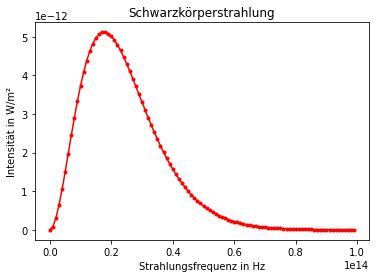
\includegraphics[width=\linewidth]{./gfx/plt-labels}
\end{tcolorbox}
\end{columns}
%
\end{frame}

% =========================================================================== %

\begin{frame}[fragile]
%
\begin{codebox}[Example: Linear and Logarithmic Plot]
\begin{minted}[linenos, fontsize=\scriptsize]{python3}
import matplotlib.pyplot as plt

W  = 500
X  = [x / 10 for x in range(-W, W)]
Y1 = [2 ** x for x in X]
Y2 = [x ** 7 for x in X]

plt.title("Linear Plot")
plt.plot(X, Y1, label="exponential")
plt.plot(X, Y2, label="power")
plt.legend()
plt.show()

plt.title("Logarithmic Plot")
plt.yscale("log")
plt.plot(X, Y1, label="exponential")
plt.plot(X, Y2, label="power")
plt.legend()
plt.show()
\end{minted}
\end{codebox}
%
\end{frame}

% =========================================================================== %

\begin{frame}[fragile]
%
\begin{tcbraster}[raster columns=2,
                  raster equal height,
                  nobeforeafter,
                  raster column skip=0.5cm]
\begin{tcolorbox}[title=Linear Plot]
	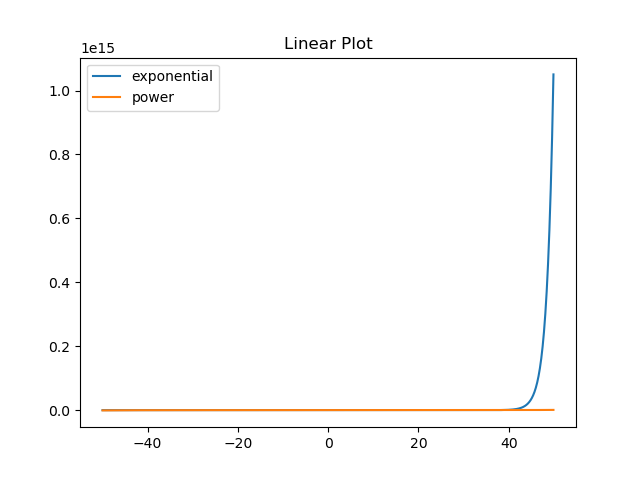
\includegraphics[width=\linewidth]{./gfx/plt-linear}
\end{tcolorbox}
%
\begin{tcolorbox}[title=Logarithmic Plot]
	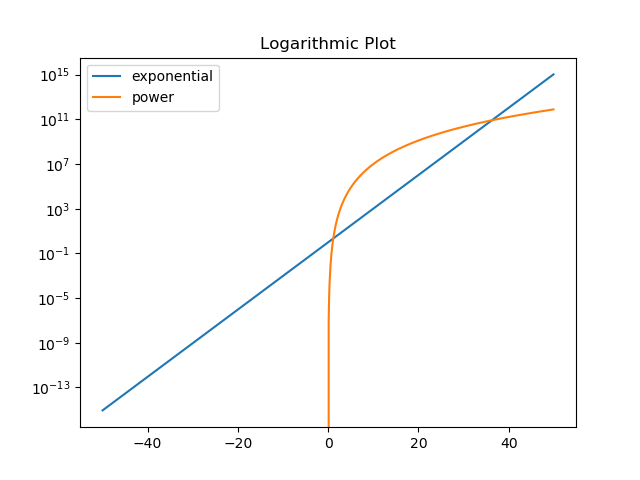
\includegraphics[width=\linewidth]{./gfx/plt-logarithmic}
\end{tcolorbox}
\end{tcbraster}
%
\end{frame}

% =========================================================================== %

\begin{frame}[fragile]{Logarithmic plots}
%
\begin{itemize}
\item Distort one or both axes to show highly dynamic processes
\item Equal distance -- constant factor
\item Doesn't work for negative values
\item Alternative: \inPy{"symlog"}
	\begin{itemize}
	\item \emph{symmetric logarithmic}
	\item Above [limit] and below -[limit]: logarithmic projection
	\item Between -[limit] and +[limit]: \emph{linear} projection
	\item limit: optional parameters \texttt{linthreshx} or \texttt{linthreshy}, respectively
	\end{itemize}
\end{itemize}
%
\end{frame}

% =========================================================================== %

\begin{frame}[fragile]
%
\begin{codebox}[Example: Symmetric Logarithmic Plots]
\begin{minted}[linenos, fontsize=\scriptsize]{python3}
import math
import matplotlib.pyplot as plt

W  = 500
X  = [x / 10 for x in range(-W, W)]
Y1 = [math.sin(x) for x in X]
Y2 = [x / 10      for x in X]

plt.xscale("symlog")
plt.plot(X, Y1)
plt.plot(X, Y2)
plt.grid()
plt.show()

plt.xscale("symlog", linthreshx=10)
plt.plot(X, Y1)
plt.plot(X, Y2)
plt.grid()
plt.show()
\end{minted}
\end{codebox}
%
\end{frame}

% =========================================================================== %

\begin{frame}[fragile]
%
\begin{tcbraster}[raster columns=2,
                  raster equal height,
                  nobeforeafter,
                  raster column skip=0.5cm]
\begin{tcolorbox}[title=symlog{,} default threshold]
	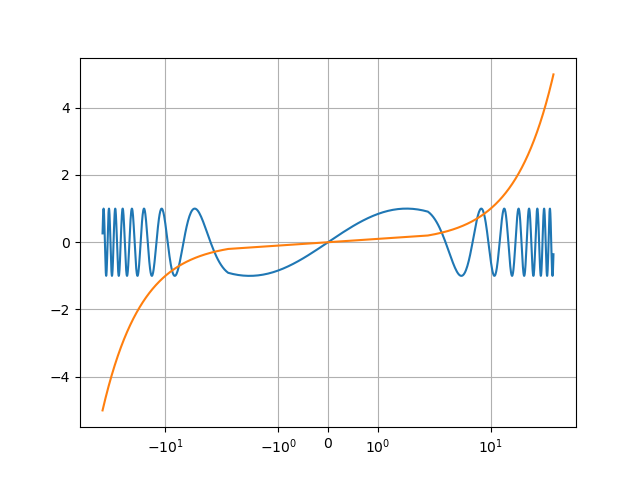
\includegraphics[width=\linewidth]{./gfx/plt-symlog}
\end{tcolorbox}
%
\begin{tcolorbox}[title=symlog{,} explicit threshold]
	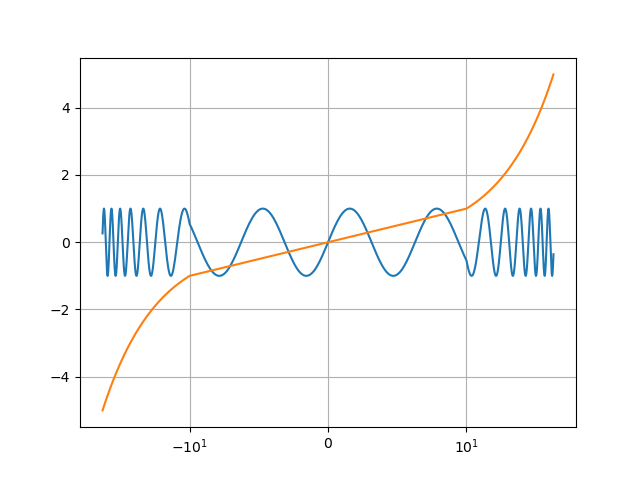
\includegraphics[width=\linewidth]{./gfx/plt-symlog-threshold}
\end{tcolorbox}
\end{tcbraster}
%
\end{frame}

% =========================================================================== %

\begin{frame}[fragile]
%
\begin{codebox}[Example: Manually Scaled Axes, width=.53\linewidth, nobeforeafter, equal height group = grpXmpSimplePlotScale]
\begin{minted}[linenos, fontsize=\scriptsize]{python3}
import math
import matplotlib.pyplot as plt

N = 100
X = [(x - N/2) / 10 for x in range(N)]
Y = [math.sin(x) for x in X]

plt.plot(X, Y)
plt.xlim(-6  , +6)
plt.ylim(-0.7, +3)
plt.grid()
plt.show()
\end{minted}
\end{codebox}
%
\begin{tcolorbox}[title=Output: Manually Scaled Axes, width=.45\linewidth, nobeforeafter, equal height group = grpXmpSimplePlotScale]
	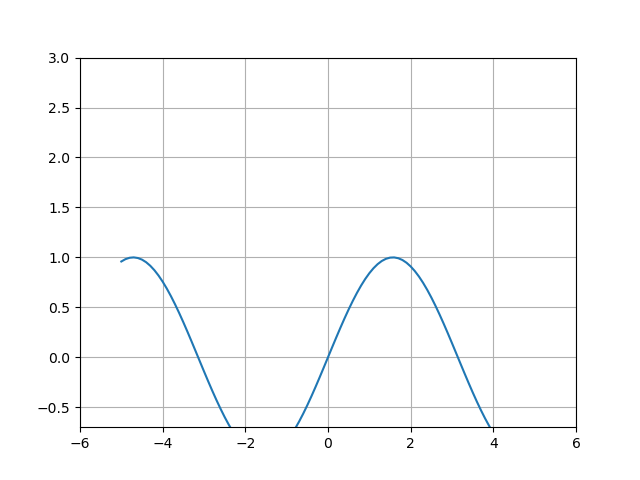
\includegraphics[width=\linewidth]{./gfx/plt-limits}
\end{tcolorbox}
%
\end{frame}

% =========================================================================== %
\end{document}

% MAREI!!
% whom do I give credit? Where?